\chapter{Pushdown Automater og Kontekstfrie Sprog}

Kontekstfrie Sprog er en klasse af sprog, som beskrives af hhv. Pushdown Automater og Kontekstfrie Grammatikker. Denne klasse af sprog er ``større'', det vil sige, indeholder flere mulige sprog end klassen af regulære sprog.

\section{Kontekstfrie Grammatikker}%
\label{sec:label}

\begin{definition}[Kontekstfri Grammatik]
  En kontekstfri grammatik er en 4-tuple $G = (V, \Sigma, R, S)$, hvor:
  \begin{itemize}
    \item $V$ er variablerne,
    \item $\Sigma$ er et endeligt alfabet,
    \item $R$ er substitueringsreglerne,
    \item $S$ er startsymbolet.
  \end{itemize}
\end{definition}

En \textit{afledning} $S \Rightarrow u_{1}A_{1}v_{1} \Rightarrow u_{2}A_{2}v_{2} \Rightarrow \cdots \Rightarrow u_{k}A_{k}v_{k} \Rightarrow w \in \Sigma^{*}$. Hvert skridt erstatter en variabel $A_{i}$ med højrehåndssiden af en regel i $R$. Vi skriver $S \stackrel{*}{\Rightarrow} w$ hvis $S$ kan aflede $w$ i en eller flere skridt. $L(G) = \{w \in \Sigma^{*} \mid S \stackrel{*}{\Rightarrow} w\}$.

Vi kalder denne sprogklasse \textit{kontekstfri}, da en erstatning af et symbol $A$ i f.eks. $uAv$ hvor $A \rightarrow \delta \in R$ ikke afhænger af $u$ af $v$, altså konteksten.

Uden at gå ind i detaljerne for hvad et parsetræ er, udover en grafisk forklaring på hvordan man afleder (eller udleder, jeg er ærligt i tvivl) en streng fra et symbol, kan man se et eksempel i Figur~\ref{fig:parsetreeg1} for følgende kontekstrfrie grammatik:

\begin{equation}
	\tag{$G_{1}$}
	\begin{split}
		A & \rightarrow \mathtt{0}A \mathtt{1} \\
		A & \rightarrow B                      \\
		B & \rightarrow \mathtt{\#}
	\end{split}
	\label{eqn:G1}
\end{equation}

\begin{figure}[ht]
	\centering
	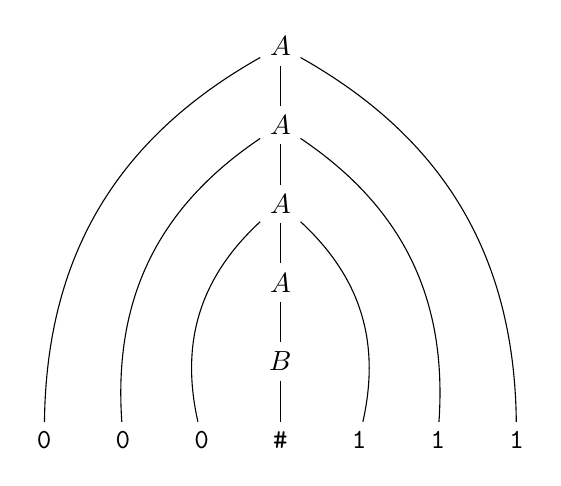
\begin{tikzpicture}[>=latex]
		% Nodes
		\node (0a) at (0,0) {\texttt{0}};
		\node (0b) at (1,0) {\texttt{0}};
		\node (0c) at (2,0) {\texttt{0}};
		\node (sharp) at (3,0) {\texttt{\#}};
		\node (1a) at (4,0) {\texttt{1}};
		\node (1b) at (5,0) {\texttt{1}};
		\node (1c) at (6,0) {\texttt{1}};

		% Upper nodes
		\node (B) at (3,1) {$B$};
		\node (A4) at (3,2) {$A$};
		\node (A3) at (3,3) {$A$};
		\node (A2) at (3,4) {$A$};
		\node (A1) at (3,5) {$A$};

		% Lines going down
		\draw[-] (B) to (sharp);
		\draw[-] (A4) to (B);
		\draw[-] (A3) to (A4);
		\draw[-] (A2) to (A3);
		\draw[-] (A1) to (A2);

		% Lines going to terminals
		\draw[-] (A1) to[bend right] (0a);
		\draw[-] (A1) to[bend left] (1c);
		\draw[-] (A2) to[bend right] (0b);
		\draw[-] (A2) to[bend left] (1b);
		\draw[-] (A3) to[bend right] (0c);
		\draw[-] (A3) to[bend left] (1a);

	\end{tikzpicture}
	\caption{\label{fig:parsetreeg1} Parse-træ for \texttt{000\#111} i \eqref{eqn:G1}}
\end{figure}

% 04:34


%%% Local Variables:
%%% mode: latex
%%% TeX-engine: xetex
%%% TeX-command-extra-options: "-shell-escape"
%%% TeX-master: "main"
%%% End:
